% ============================================================
%  يُترجَم بـ XeLaTeX  (في Overleaf: Menu → Compiler → XeLaTeX)
%  الخط: Amiri (متوفر في Overleaf، أو حمّله من github.com/aliftype/amiri)
% ============================================================
\documentclass[12pt,a4paper]{article}
\usepackage[a4paper,margin=1.7cm,top=2.3cm,bottom=2.9cm,headheight=15pt,footskip=1.5cm]{geometry}
\usepackage{amsmath,amssymb}
\usepackage{icomma}
\usepackage[english,bidi=default,layout=lists]{babel}
\babelprovide[import,main]{arabic}
\babelfont{rm}[Scale=1.08]{Amiri}
\babelfont{sf}[Scale=1.08]{Amiri}
\usepackage[most]{tcolorbox}
\usepackage{tikz}
\usetikzlibrary{arrows.meta,calc,shadings}
\usepackage{array}
\usepackage{colortbl}
\usepackage{fancyhdr}
\usepackage{titlesec}
\usepackage{enumitem}
\usepackage{collcell}
\usepackage{needspace}
\usepackage{etoolbox}
\newcolumntype{C}{>{\collectcell\ar}c<{\endcollectcell}}
\pretocmd{\section}{\Needspace{15\baselineskip}}{}{}
\pretocmd{\subsection}{\Needspace{11\baselineskip}}{}{}

\definecolor{cDef}{HTML}{1F4E9C}
\definecolor{cThm}{HTML}{B3261E}
\definecolor{cRem}{HTML}{2E7D32}
\definecolor{cEx}{HTML}{C76B00}
\definecolor{cMeth}{HTML}{6A1B9A}
\definecolor{cSol}{HTML}{00695C}
\definecolor{cSec}{HTML}{1F3A68}

\titleformat{\section}{\Large\bfseries\color{cSec}}{\thesection.}{0.6em}{}[{\color{cSec!60}\titlerule[1pt]}]
\titleformat{\subsection}{\large\bfseries\color{cThm!85!black}}{\thesubsection.}{0.5em}{}
\titlespacing*{\section}{0pt}{14pt}{8pt}
\titlespacing*{\subsection}{0pt}{10pt}{5pt}
\setlength{\parindent}{0pt}
\setlength{\parskip}{4pt}
\setlist{itemsep=2pt,topsep=3pt}

\newtcolorbox{arbox}[3][]{enhanced,
  colback=#2!5,colframe=#2!80!black,arc=2mm,boxrule=0.8pt,
  left=6pt,right=6pt,top=8pt,bottom=5pt,
  fonttitle=\bfseries,coltitle=white,
  title={\foreignlanguage{arabic}{#3}},
  attach boxed title to top right={xshift=-5mm,yshift=-3mm},
  boxed title style={colback=#2!80!black,arc=1.5mm,boxrule=0pt},
  before upper={\selectlanguage{arabic}},
  before skip=8pt,after skip=8pt,breakable,#1}
\newenvironment{BOX}[2]{\begin{otherlanguage}{english}\begin{arbox}{#1}{#2}}{\end{arbox}\end{otherlanguage}}
\newenvironment{tarif}[1][تعريف]{\begin{BOX}{cDef}{#1}}{\end{BOX}}
\newenvironment{khassia}[1][خاصية]{\begin{BOX}{cThm}{#1}}{\end{BOX}}
\newenvironment{molahada}[1][ملاحظة]{\begin{BOX}{cRem}{#1}}{\end{BOX}}
\newenvironment{mithal}[1][مثال]{\begin{BOX}{cEx}{#1}}{\end{BOX}}
\newenvironment{tariqa}[1][طريقة]{\begin{BOX}{cMeth}{#1}}{\end{BOX}}

\newcounter{exo}
\newenvironment{tamrin}[1]{\stepcounter{exo}\begin{BOX}{cSec}{التمرين \theexo: #1}}{\end{BOX}}
\newenvironment{hal}{\Needspace{12\baselineskip}\begin{otherlanguage}{english}\begin{arbox}[breakable]{cSol}{حل التمرين \theexo}}{\end{arbox}\end{otherlanguage}}

\newenvironment{LTR}{\begin{otherlanguage}{english}}{\end{otherlanguage}}
\newcommand{\ar}[1]{\foreignlanguage{arabic}{#1}}

\renewcommand{\dots}{\mathinner{\ldotp\ldotp\ldotp}}
\renewcommand{\ldots}{\mathinner{\ldotp\ldotp\ldotp}}
\renewcommand{\cdots}{\mathinner{\cdotp\cdotp\cdotp}}
\newcommand{\N}{\mathbb{N}}
\newcommand{\Z}{\mathbb{Z}}
\newcommand{\D}{\mathbb{D}}
\newcommand{\Q}{\mathbb{Q}}
\newcommand{\R}{\mathbb{R}}
\newcommand{\pgcd}{\operatorname{PGCD}}
\newcommand{\ppcm}{\operatorname{PPCM}}

% \NLseg{a}{b}{[}{]} ; \NLright{a}{[} ; \NLleft{b}{]}  (interval on a number line)
\newcommand{\NLseg}[4]{\begin{LTR}\begin{tikzpicture}[baseline=-0.6ex]
 \draw[-{Stealth[length=2mm]},gray!70](0,0)--(3.4,0);
 \draw[line width=2pt,cThm!80!black](0.7,0)--(2.7,0);
 \node[cThm!80!black,font=\LARGE] at (0.7,0){$#3$};
 \node[cThm!80!black,font=\LARGE] at (2.7,0){$#4$};
 \node[below=3pt,font=\footnotesize] at (0.7,0){$#1$};
 \node[below=3pt,font=\footnotesize] at (2.7,0){$#2$};
\end{tikzpicture}\end{LTR}}
\newcommand{\NLright}[2]{\begin{LTR}\begin{tikzpicture}[baseline=-0.6ex]
 \draw[-{Stealth[length=2mm]},gray!70](0,0)--(3.4,0);
 \draw[line width=2pt,cThm!80!black](1.3,0)--(3.3,0);
 \node[cThm!80!black,font=\LARGE] at (1.3,0){$#2$};
 \node[below=3pt,font=\footnotesize] at (1.3,0){$#1$};
\end{tikzpicture}\end{LTR}}
\newcommand{\NLleft}[2]{\begin{LTR}\begin{tikzpicture}[baseline=-0.6ex]
 \draw[-{Stealth[length=2mm]},gray!70](0,0)--(3.4,0);
 \draw[line width=2pt,cThm!80!black](0.05,0)--(2.1,0);
 \node[cThm!80!black,font=\LARGE] at (2.1,0){$#2$};
 \node[below=3pt,font=\footnotesize] at (2.1,0){$#1$};
\end{tikzpicture}\end{LTR}}

% ---------- social-media icons (pure TikZ) ----------
\definecolor{cFB}{HTML}{1877F2}
\definecolor{cTG}{HTML}{229ED9}
\definecolor{cIG1}{HTML}{FEDA75}
\definecolor{cIG2}{HTML}{D62976}
\definecolor{cIG3}{HTML}{4F5BD5}
\newcommand{\fbicon}{\begin{LTR}\begin{tikzpicture}[baseline=-0.75ex,x=1em,y=1em]
 \fill[cFB] (0,0) circle (0.55);
 \node[white,inner sep=0,font=\usefont{TU}{lmss}{bx}{n}\small] at (0.04,-0.02) {f};
\end{tikzpicture}\end{LTR}}
\newcommand{\igicon}{\begin{LTR}
\begin{tikzpicture}[baseline=-0.75ex,x=1em,y=1em]
 \shade[lower left=cIG1,lower right=cIG2,upper left=cIG2,upper right=cIG3,rounded corners=0.28em] (-0.55,-0.55) rectangle (0.55,0.55);
 \draw[white,line width=0.09em,rounded corners=0.18em] (-0.36,-0.36) rectangle (0.36,0.36);
 \draw[white,line width=0.09em] (0,0) circle (0.17);
 \fill[white] (0.22,0.22) circle (0.05);
\end{tikzpicture}\end{LTR}}
\newcommand{\tgicon}{\begin{LTR}
\begin{tikzpicture}[baseline=-0.75ex,x=1em,y=1em]
 \fill[cTG] (0,0) circle (0.55);
 \fill[white] (-0.33,0.0) -- (0.32,0.27) -- (0.2,-0.3) -- (0.0,-0.15) -- (-0.08,-0.28) -- (-0.08,-0.08) -- cycle;
 \fill[cTG!70!black] (-0.08,-0.08) -- (0.25,0.2) -- (0.0,-0.15) -- (-0.08,-0.28) -- cycle;
\end{tikzpicture}\end{LTR}}
% page number: black box, white two-digit number, at the right of the social row
\newcommand{\PageBox}{\begin{LTR}\tikz[baseline=(p.base)]\node[fill=black,text=white,inner sep=2.5pt,minimum width=1.6em,minimum height=1.3em,font=\usefont{TU}{lmss}{bx}{n}\small](p){\ifnum\value{page}<10 0\fi\arabic{page}};\end{LTR}}
% visual left-to-right order: Telegram | Instagram | Facebook | page box
\newcommand{\SocialRow}{\begin{otherlanguage}{english}%
 \ar{\textbf{الأستاذ سوايسية هشام للرياضيات}}\ \tgicon\hfill
 \textbf{prof\_hicham\_math}\ \igicon\hfill
 \ar{\textbf{الأستاذ سوايسية هشام للرياضيات}}\ \fbicon\hspace{2.2em}\PageBox\end{otherlanguage}}

\pagestyle{fancy}
\fancyhf{}
\renewcommand{\headrulewidth}{0.6pt}
\renewcommand{\footrulewidth}{0.4pt}
% \SetHeader{right head: document title}{left head: level -- stream}
\newcommand{\SetHeader}[2]{%
 \fancyhead[C]{\parbox{\textwidth}{\ar{#1\hfill #2}}}%
 \fancyfoot[C]{\parbox{\textwidth}{\small\SocialRow}}}
\usepackage{tkz-tab}
\usepackage{multicol}
% variation / sign table (LTR)
\newenvironment{TAB}{\par\begin{center}\begin{LTR}\begin{tikzpicture}[scale=0.95,every node/.style={font=\small}]}{\end{tikzpicture}\end{LTR}\end{center}}
% grid + axes, clipped: \begin{GR}{xmin}{xmax}{ymin}{ymax}{unit cm}
\newenvironment{GR}[5]{\par\begin{center}\begin{LTR}\begin{tikzpicture}[x=#5cm,y=#5cm,font=\footnotesize]
 \draw[gray!25,very thin] (#1,#3) grid (#2,#4);
 \draw[-{Stealth[length=2mm]}] (#1,0)--(#2+0.3,0) node[below left]{$x$};
 \draw[-{Stealth[length=2mm]}] (0,#3)--(0,#4+0.3) node[below left]{$y$};
 \node[below left] at (0,0){$O$};
 \begin{scope}\clip (#1,#3) rectangle (#2,#4);}
{\end{scope}\end{tikzpicture}\end{LTR}\end{center}}
\newcommand{\Ticks}[2]{\foreach \t in {#1} \node[below,font=\scriptsize] at (\t,0){$\t$}; \foreach \t in {#2} \node[left,font=\scriptsize] at (0,\t){$\t$};}
\newcommand{\bx}[1]{\ensuremath{\colorbox{cDef!12}{$\displaystyle #1$}}}
\newcommand{\TwoCol}[4]{\par\begin{LTR}\noindent\begin{minipage}[t]{#1\textwidth}\selectlanguage{arabic}#2\end{minipage}\hfill\begin{minipage}[t]{#3\textwidth}\selectlanguage{arabic}#4\end{minipage}\end{LTR}\par}
\newcommand{\RL}[4]{\TwoCol{#3}{#4}{#1}{#2}}  % \RL{w1}{right content}{w2}{left content}
\newcommand{\ok}{$\textcolor{cRem}{\checkmark}$}
\newcommand{\limn}{\displaystyle\lim_{n\to+\infty}}
% sub-questions, each on its own line
\newenvironment{sq}{\begin{itemize}[leftmargin=2.4em,itemsep=3pt]}{\end{itemize}}
\newcommand{\qa}{\item[(أ)]}\newcommand{\qb}{\item[(ب)]}\newcommand{\qc}{\item[(جـ)]}\newcommand{\qd}{\item[(د)]}\newcommand{\qe}{\item[(هـ)]}
\newcommand{\pa}{\par\smallskip\textbf{(أ)} }\newcommand{\pb}{\par\smallskip\textbf{(ب)} }\newcommand{\pc}{\par\smallskip\textbf{(جـ)} }\newcommand{\pd}{\par\smallskip\textbf{(د)} }\newcommand{\pe}{\par\smallskip\textbf{(هـ)} }
\newcommand{\QQ}[1]{\par\smallskip\textbf{#1.} }
\newenvironment{tmr}{\stepcounter{exo}\begin{BOX}{cSec}{تمرين محلول \theexo}}{\end{BOX}}
\newcommand{\ABC}[3]{\\[2pt]\begin{tabular}{p{0.28\textwidth}p{0.28\textwidth}p{0.28\textwidth}}(جـ) \ #3 & (ب) \ #2 & (أ) \ #1\end{tabular}}
\pretocmd{\section}{\Needspace{24\baselineskip}}{}{}
\newtcbox{\bxtbox}{on line,colback=cDef!12,colframe=cDef!12,boxrule=0pt,arc=1pt,boxsep=0pt,left=2pt,right=2pt,top=1pt,bottom=1pt}
\newcommand{\bxt}[1]{\foreignlanguage{english}{\bxtbox{\ar{#1}}}}
\usepackage{longtable}
\setlength{\LTpre}{4pt}\setlength{\LTpost}{0pt}
\newcommand{\Phase}[1]{\textbf{#1}}
\newcommand{\Fld}[2]{\textbf{#1:}\ #2}
% رأس المذكرة على نمط النموذج: إطار بعنوان «مذكرة رقم»، معلومات الحصة، ثم إطار الكفاءات
\newcommand{\ModhHead}[9]{%
\begin{LTR}
\begin{tcolorbox}[enhanced,colback=white,colframe=cThm!85!black,arc=4mm,boxrule=1pt,top=14pt,bottom=6pt,left=8pt,right=8pt,
 overlay={\node[fill=cThm!85!black,text=white,rounded corners=3mm,inner xsep=14pt,inner ysep=4pt,font=\large\bfseries] at ([yshift=0pt]frame.north){\ar{مذكرة رقم #1}};},
 before upper={\selectlanguage{arabic}}]
\begin{tabular}{@{}p{0.4\linewidth}p{0.55\linewidth}@{}}
\Fld{المستوى}{#2} & \Fld{الثانوية}{\dotfill}\\[3pt]
\Fld{المادة}{رياضيات} & \Fld{ميدان التعلم}{#3}\\[3pt]
\Fld{المدة}{#5} & \Fld{الوحدة التعلمية}{#4}\\[3pt]
\Fld{الأستاذ}{\dotfill} & \Fld{المحتوى المعرفي}{#6}\\
\end{tabular}
\end{tcolorbox}
\begin{tcolorbox}[enhanced,colback=white,colframe=cThm!85!black,arc=3mm,boxrule=0.8pt,sidebyside,sidebyside align=top,lefthand ratio=0.5,
 segmentation style={dashed,cThm!60},before upper={\selectlanguage{arabic}},before lower={\selectlanguage{arabic}}]
\textbf{الكفاءات المستهدفة:}\par #8
\tcblower
\textbf{الكفاءات القبلية:}\par #7
\end{tcolorbox}
\end{LTR}
\par\smallskip\textbf{الوسائل:} #9\par\smallskip}
\newenvironment{Sayr}{%
\begin{LTR}\renewcommand{\arraystretch}{1.25}
\begin{longtable}{|p{0.17\textwidth}|>{\centering\arraybackslash}p{0.06\textwidth}|p{0.53\textwidth}|>{\centering\arraybackslash}p{0.12\textwidth}|}
\hline\rowcolor{cThm!12}\ar{\textbf{توجيهات وتعاليق}} & \ar{\textbf{المدة}} & \ar{\textbf{سير الحصة}} & \ar{\textbf{مراحل الحصة}}\\\hline\endhead
\hline\endfoot}{\end{longtable}\end{LTR}}
% سطر في الجدول: \Row{مرحلة}{سير}{مدة}{توجيهات}
\newcommand{\Row}[4]{\ar{\small #4} & \ar{#3} & \ar{#2} & \cellcolor{cThm!8}\ar{\Phase{#1}}\\\hline}

\newcommand{\Lab}[2]{\foreignlanguage{english}{\tcbox[on line,colback=#1,colframe=#1,boxrule=0pt,arc=2pt,boxsep=1pt,left=5pt,right=5pt,top=1pt,bottom=1pt]{\ar{\textcolor{white}{\textbf{#2}}}}}}
\newcommand{\Num}[1]{\foreignlanguage{english}{\tikz[baseline=(c.base)]\node[fill=cDef,text=white,inner sep=2pt,font=\footnotesize\bfseries](c){#1};}}
\newcommand{\ck}{\ensuremath{{\color{cRem}\checkmark}}}
\newenvironment{Kad}[1]{\par\smallskip\Lab{#1}}{\par}
\SetHeader{\small\bfseries\color{cSec}مذكرات محور: العبارات الجبرية}{\small\color{cSec}السنة الأولى ثانوي -- جذع مشترك علوم وتكنولوجيا}
\begin{document}
\begin{LTR}
\begin{tcolorbox}[enhanced,colback=cThm!85!black,colframe=cThm!85!black,arc=3mm,halign=center,boxrule=0pt,top=12pt,bottom=12pt,before upper={\selectlanguage{arabic}}]
{\color{white}\fontsize{26}{32}\selectfont\bfseries مذكرات محور: العبارات الجبرية}\\[8pt]
{\color{white}\large السنة الأولى ثانوي -- جذع مشترك علوم وتكنولوجيا}\\[4pt]
{\color{white}\large 7 مذكرات (14 ساعة) -- السنة الدراسية 2026-2027}
\end{tcolorbox}
\end{LTR}
\begin{BOX}{cThm}{يتضمن هذا العمل}
\begin{enumerate}[label=\textbf{مذكرة \arabic{enumi}:},leftmargin=6em,start=29]
\item العبارات الجبرية: أشكالها وقيمتها العددية.
\item تحويل عبارة جبرية: النشر ، التحليل ، المتطابقات الشهيرة.
\item الشكل النموذجي لثلاثي حدود من الدرجة الثانية.
\item حل المعادلة $ax^2+bx+c=0$ ، المميز.
\item حل المعادلات والمتراجحات جبرياً.
\item حل المعادلات والمتراجحات بيانياً.
\item ترييض المشكلات.
\end{enumerate}
مراجع النشاطات: الكتاب المدرسي للسنة الأولى ثانوي جذع مشترك علوم وتكنولوجيا (باب المعادلات والمتراجحات ص 112--114).
\end{BOX}
\newpage
\ModhHead{29}{1 ج م ع ت}{جبر}{العبارات الجبرية}{02 سا}{العبارات الجبرية: أشكالها وقيمتها العددية}%
{\begin{itemize}\item الحساب الحرفي (التعليم المتوسط).\item قواعد الحساب على الكسور.\end{itemize}}%
{\begin{itemize}\item التعرّف على الصيغ المختلفة لنفس العبارة.\item حساب القيمة العددية لعبارة وتعيين القيم الممنوعة.\end{itemize}}%
{المنهاج ، الكتاب المدرسي ، مراجع ، الحاسبة البيانية.}
\begin{Sayr}
\Row{مرحلة الانطلاق}{%
\textbf{التهيئة النفسية:} ثمن $x$ كراريس بـ $45$ DA وقلمين بـ $30$ DA: اكتب الثمن الكلي. هل يمكن كتابته بطريقة أخرى؟}{10 د}{وضعية من الحياة اليومية.}
\Row{التشخيص والاكتشاف}{%
\Lab{cEx}{مناقشة نشاط 01 صفحة 112}\par\ck\ $ab+cd$ \textbf{مجموع} جداءين ؛ $(a+b)(c+d)$ \textbf{جداء} مجموعين ؛ $\dfrac{ab}{c+d}$ حاصل قسمة جداء على مجموع.\par
\ck\ $\dfrac{1}{a+b}$ معرفة فقط إذا كان $a+b\ne0$.\par
\ck\ نسمي العبارة حسب \textbf{آخر عملية} نجريها في الحساب.\par
}{35 د}{عمل فردي على الجدول.}
\Row{بناء المعارف}{%
\Lab{cDef}{تعريف}\ \textbf{العبارة الجبرية} كتابة تحتوي أعداداً وحروفاً مرتبطة بعمليات. \textbf{قيمتها العددية} هي العدد الناتج عند تعويض الحروف بأعداد.\par\Lab{cEx}{مثال}\par\ck\ $E(x)=2x^2-3x+5$: من أجل $x=-1$: $E(-1)=2+3+5=10$.\par
\ck\ $A=3(2x-1)^2$ \textbf{جداء} ؛ $B=2-x(x+1)$ \textbf{فرق} ؛ $C=\dfrac{1}{x-3}+2$ \textbf{مجموع}.\par
}{50 د}{نشدد على أولوية العمليات.}
\Row{}{%
\Lab{cRem}{القيم الممنوعة}\ $B(x)=\dfrac{x+2}{x-2}$ ليس لها قيمة عددية من أجل $x=2$: نقول إن $2$ \textbf{قيمة ممنوعة}.\par\Lab{cThm!80!black}{حذار}\ $-x^2$ من أجل $x=-3$ تساوي $-9$ وليس $9$.}{}{}
\Row{التقويم}{%
\Lab{cEx}{تطبيق}\par\Num{1} احسب $F(x)=\dfrac{x^2-1}{x+3}$ من أجل $x=0$ و $x=1$. ما القيمة الممنوعة؟ \Num{2} سمّ العبارة $(1-x)\sqrt x$.\par\textbf{الحل:} \Num{1} $F(0)=-\dfrac13$ ، $F(1)=0$ ، القيمة الممنوعة $-3$ ؛ \Num{2} جداء.\par\textbf{واجب منزلي:} تمارين من الكتاب المدرسي.\par\smallskip\textbf{ملاحظات حول سير الحصة:} \dotfill}{25 د}{تقويم فردي.}
\end{Sayr}
\newpage
\ModhHead{30}{1 ج م ع ت}{جبر}{العبارات الجبرية}{02 سا}{تحويل عبارة جبرية: النشر ، التحليل ، المتطابقات الشهيرة}%
{\begin{itemize}\item النشر والتحليل (المتوسط).\end{itemize}}%
{\begin{itemize}\item نشر وتحليل واختصار عبارة جبرية.\item استعمال المتطابقات الشهيرة.\end{itemize}}%
{المنهاج ، الكتاب المدرسي ، مراجع ، الحاسبة البيانية.}
\begin{Sayr}
\Row{مرحلة الانطلاق}{%
\textbf{التهيئة النفسية:} احسب ذهنياً: $99^2$ ؛ $101\times99$.}{10 د}{حساب ذهني بالمتطابقات.}
\Row{التشخيص والاكتشاف}{%
\Lab{cEx}{مناقشة نشاط 02 صفحة 112}\par\ck\ مساحة مربع ضلعه $a+b$ تساوي مجموع مساحات أربع قطع: $(a+b)^2=a^2+2ab+b^2$.\par
\ck\ بنفس الطريقة: $(a-b)^2=a^2-2ab+b^2$ و $(a-b)(a+b)=a^2-b^2$.\par
\ck\ $399^2=(400-1)^2=160000-800+1=159201$.\par
}{35 د}{نرسم المربع المقسم على السبورة.}
\Row{بناء المعارف}{%
\Lab{cThm}{المتطابقات الشهيرة}\ $(a+b)^2=a^2+2ab+b^2$ ؛ $(a-b)^2=a^2-2ab+b^2$ ؛ $(a-b)(a+b)=a^2-b^2$.\par\Lab{cDef}{تعريف}\ \textbf{النشر}: تحويل جداء إلى مجموع ؛ \textbf{التحليل}: تحويل مجموع إلى جداء.\par}{50 د}{نلخص المتطابقات في إطار.}
\Row{}{%
\Lab{cEx}{مثال}\par\ck\ $(2x-3)^2=4x^2-12x+9$.\par
\ck\ $9x^2-16=(3x-4)(3x+4)$ ؛ $x^2-6x+9=(x-3)^2$.\par
\ck\ عامل مشترك: $(x+1)(2x-3)-(x+1)(x+4)=(x+1)(x-7)$.\par
\Lab{cMeth}{اختصار كسر}\ نحلل البسط والمقام ثم نختصر بشرط: $\dfrac{x^2-1}{x+1}=x-1$ من أجل $x\ne-1$.\par}{}{}
\Row{}{%
\Lab{cThm!80!black}{حذار}\ $(a+b)^2\ne a^2+b^2$.}{}{}
\Row{التقويم}{%
\Lab{cEx}{تطبيق}\par\Num{1} انشر $(x+2)(x-5)$. \Num{2} حلّل $4x^2-12x+9$ و $(x-1)^2-9$.\par\textbf{الحل:} \Num{1} $x^2-3x-10$ ؛ \Num{2} $(2x-3)^2$ ؛ $(x-4)(x+2)$.\par\textbf{واجب منزلي:} تمارين من الكتاب المدرسي.\par\smallskip\textbf{ملاحظات حول سير الحصة:} \dotfill}{25 د}{تقويم فردي.}
\end{Sayr}
\newpage
\ModhHead{31}{1 ج م ع ت}{جبر}{العبارات الجبرية}{02 سا}{الشكل النموذجي لثلاثي حدود من الدرجة الثانية}%
{\begin{itemize}\item المتطابقات الشهيرة.\item التحليل.\end{itemize}}%
{\begin{itemize}\item كتابة ثلاثي حدود على الشكل النموذجي.\item استعمال الشكل النموذجي للتحليل وتعيين قيمة حدية.\end{itemize}}%
{المنهاج ، الكتاب المدرسي ، مراجع ، الحاسبة البيانية.}
\begin{Sayr}
\Row{مرحلة الانطلاق}{%
\textbf{التهيئة النفسية:} أكمل ليكون مربعاً تاماً: $x^2+6x+\ldots$ ؛ $x^2-10x+\ldots$}{10 د}{لعبة إكمال المربع.}
\Row{التشخيص والاكتشاف}{%
\Lab{cEx}{مناقشة نشاط 03 صفحة 113 ونشاط 04 صفحة 114}\par\ck\ الخوارزمي يحل $x^2+21=10x$ هندسياً: $x^2-10x+21=(x-5)^2-4$ ، إذن $(x-5)^2=4$ ، أي $x=3$ أو $x=7$.\par
\ck\ هرم خوفو: $\varphi^2-\varphi-1=\Big(\varphi-\dfrac12\Big)^2-\dfrac54=0$ ، إذن $\varphi=\dfrac{1+\sqrt5}{2}\approx1{,}618$ (\textbf{العدد الذهبي}).\par
}{35 د}{لمحة تاريخية: الخوارزمي والعدد الذهبي.}
\Row{بناء المعارف}{%
\Lab{cThm}{خاصية}\ من أجل $a\ne0$: \ $ax^2+bx+c=a\Big[\Big(x+\dfrac{b}{2a}\Big)^2-\dfrac{b^2-4ac}{4a^2}\Big]$: هذا هو \textbf{الشكل النموذجي}.\par\Lab{cMeth}{طريقة}\ نخرج $a$ عاملاً ، ثم نكمل المربع: $x^2+px=\Big(x+\dfrac p2\Big)^2-\dfrac{p^2}4$.\par}{50 د}{نكتب الطريقة خطوة خطوة.}
\Row{}{%
\Lab{cEx}{مثال}\par\ck\ $2x^2+4x-6=2\big[(x+1)^2-4\big]=2(x-1)(x+3)$.\par
\ck\ $x^2-4x+7=(x-2)^2+3\geqslant3$: القيمة الحدية الصغرى $3$ عند $x=2$.\par
\Lab{cThm!80!black}{حذار}\ لا ننسى إخراج $a$ قبل إكمال المربع.}{}{}
\Row{التقويم}{%
\Lab{cEx}{تطبيق}\par\Num{1} اكتب $x^2+6x+5$ على الشكل النموذجي ثم حلّله. \Num{2} عيّن القيمة الحدية لـ $-x^2+2x+3$.\par\textbf{الحل:} \Num{1} $(x+3)^2-4=(x+1)(x+5)$ ؛ \Num{2} $4-(x-1)^2$: عظمى $4$ عند $1$.\par\textbf{واجب منزلي:} تمارين من الكتاب المدرسي.\par\smallskip\textbf{ملاحظات حول سير الحصة:} \dotfill}{25 د}{تقويم فردي.}
\end{Sayr}
\newpage
\ModhHead{32}{1 ج م ع ت}{جبر}{العبارات الجبرية}{02 سا}{حل المعادلة $ax^2+bx+c=0$ ، المميز}%
{\begin{itemize}\item الشكل النموذجي.\item الجذر التربيعي.\end{itemize}}%
{\begin{itemize}\item حل معادلة من الدرجة الثانية باستعمال المميز.\item تحليل ثلاثي حدود.\end{itemize}}%
{المنهاج ، الكتاب المدرسي ، مراجع ، الحاسبة البيانية.}
\begin{Sayr}
\Row{مرحلة الانطلاق}{%
\textbf{التهيئة النفسية:} حل $(x-1)^2=9$ ، ثم $(x-1)^2=0$ ، ثم $(x-1)^2=-4$.}{10 د}{ثلاث حالات بسيطة.}
\Row{التشخيص والاكتشاف}{%
\Lab{cEx}{وضعية مقترحة}\par\ck\ من الشكل النموذجي: $ax^2+bx+c=0\iff\Big(x+\dfrac b{2a}\Big)^2=\dfrac{\Delta}{4a^2}$ حيث $\Delta=b^2-4ac$.\par
\ck\ عدد الحلول يتعلق بإشارة $\Delta$ كما في الوضعية الانطلاقية: حلان ، حل واحد ، لا حل.\par
}{35 د}{ننطلق من الشكل النموذجي.}
\Row{بناء المعارف}{%
\Lab{cDef}{تعريف}\ $\Delta=b^2-4ac$ \textbf{مميز} ثلاثي الحدود.\par\Lab{cThm}{خاصية}\par\ck\ $\Delta>0$: حلان $x_1=\dfrac{-b-\sqrt\Delta}{2a}$ و $x_2=\dfrac{-b+\sqrt\Delta}{2a}$ ، و $ax^2+bx+c=a(x-x_1)(x-x_2)$.\par
\ck\ $\Delta=0$: حل مضاعف $x_0=-\dfrac b{2a}$ ، و $ax^2+bx+c=a(x-x_0)^2$.\par
\ck\ $\Delta<0$: لا حلول ، ولا يحلل.\par
}{50 د}{جدول الحالات الثلاث.}
\Row{}{%
\Lab{cEx}{مثال}\par\ck\ $2x^2-5x+2=0$: $\Delta=9$ ، $x_1=\dfrac12$ ، $x_2=2$ ، و $2x^2-5x+2=(x-2)(2x-1)$.\par
\ck\ $x^2-6x+9=0$: $\Delta=0$ ، $x_0=3$ ؛ $x^2+x+1=0$: $\Delta=-3$: لا حلول.\par
\Lab{cThm!80!black}{حذار}\ $\Delta=b^2-4ac$ وليس $b^2-4a$ ، وننتبه لإشارة $b$.}{}{}
\Row{التقويم}{%
\Lab{cEx}{تطبيق}\par حل: \Num{1} $3x^2+2x-1=0$ ؛ \Num{2} $x^2-2x-4=0$.\par\textbf{الحل:} \Num{1} $\Delta=16$: $x=-1$ أو $x=\dfrac13$ ؛ \Num{2} $\Delta=20$: $x=1-\sqrt5$ أو $x=1+\sqrt5$.\par\textbf{واجب منزلي:} تمارين من الكتاب المدرسي.\par\smallskip\textbf{ملاحظات حول سير الحصة:} \dotfill}{25 د}{تقويم فردي.}
\end{Sayr}
\newpage
\ModhHead{33}{1 ج م ع ت}{جبر}{العبارات الجبرية}{02 سا}{حل المعادلات والمتراجحات جبرياً}%
{\begin{itemize}\item إشارة ثنائي حد.\item المميز.\end{itemize}}%
{\begin{itemize}\item حل معادلات تؤول إلى جداء أو حاصل قسمة.\item حل متراجحات باستعمال جدول الإشارة.\end{itemize}}%
{المنهاج ، الكتاب المدرسي ، مراجع ، الحاسبة البيانية.}
\begin{Sayr}
\Row{مرحلة الانطلاق}{%
\textbf{التهيئة النفسية:} متى يكون الجداء $A\times B$ معدوماً؟ متى يكون موجباً؟}{10 د}{سؤال شفهي.}
\Row{التشخيص والاكتشاف}{%
\Lab{cEx}{وضعية مقترحة}\par حل $x^2=5x$. تلميذ قسم الطرفين على $x$ ووجد $x=5$ فقط. ما رأيك؟\par\ck\ $x^2-5x=0\iff x(x-5)=0\iff x=0$ أو $x=5$: القسمة على $x$ أضاعت حلاً.\par
}{35 د}{نحلل خطأ التلميذ جماعياً.}
\Row{بناء المعارف}{%
\Lab{cThm}{خاصية}\ $A\times B=0\iff A=0$ أو $B=0$ ؛ \ $\dfrac AB=0\iff A=0$ و $B\ne0$.\par\Lab{cMeth}{المتراجحات}\ ننقل كل الحدود إلى طرف واحد ، نحلل إلى عوامل من الدرجة الأولى ، ثم ننجز جدول الإشارة.\par}{50 د}{نرسم جدول الإشارة لكل مثال.}
\Row{}{%
\Lab{cEx}{مثال}\par\ck\ $\dfrac{x+1}{x-2}=3$: $x\ne2$ ، $x+1=3x-6$ ، $x=\dfrac72$.\par
\ck\ $(x-1)(x+2)\leqslant0$: $S=[-2;1]$.\par
\ck\ $x^2-x-6<0\iff(x-3)(x+2)<0$: $S=]-2;3[$.\par
\ck\ $\dfrac{2x-4}{x+1}>0$: $S=]-\infty;-1[\cup]2;+\infty[$.\par
\Lab{cThm!80!black}{حذار}\ القيم الممنوعة لا تنتمي إلى مجموعة الحلول.}{}{}
\Row{التقويم}{%
\Lab{cEx}{تطبيق}\par حل: \Num{1} $x^2-4x\geqslant0$ ؛ \Num{2} $\dfrac{3-x}{x+2}\geqslant0$.\par\textbf{الحل:} \Num{1} $]-\infty;0]\cup[4;+\infty[$ ؛ \Num{2} $]-2;3]$.\par\textbf{واجب منزلي:} تمارين من الكتاب المدرسي.\par\smallskip\textbf{ملاحظات حول سير الحصة:} \dotfill}{25 د}{تقويم فردي.}
\end{Sayr}
\newpage
\ModhHead{34}{1 ج م ع ت}{جبر}{العبارات الجبرية}{02 سا}{حل المعادلات والمتراجحات بيانياً}%
{\begin{itemize}\item التمثيل البياني لدالة.\item القراءة البيانية.\end{itemize}}%
{\begin{itemize}\item حل معادلات ومتراجحات بيانياً.\item التحقق جبرياً من الحل البياني.\end{itemize}}%
{المنهاج ، الكتاب المدرسي ، مراجع ، الحاسبة البيانية.}
\begin{Sayr}
\Row{مرحلة الانطلاق}{%
\textbf{التهيئة النفسية:} ارسم بالحاسبة البيانية $f(x)=x^2-2x-3$. أين يقطع المنحنى محور الفواصل؟}{10 د}{استعمال الحاسبة البيانية.}
\Row{التشخيص والاكتشاف}{%
\Lab{cEx}{وضعية مقترحة}\par $f(x)=x^2-2x-3$ و $g(x)=x+1$. ارسم المنحنيين ، ثم حل بيانياً $f(x)=g(x)$ و $f(x)<g(x)$.\par\ck\ المنحنيان يتقاطعان في نقطتين فاصلتاهما $-1$ و $4$.\par
\ck\ $(C_f)$ تحت $(C_g)$ بين $-1$ و $4$: $f(x)<g(x)\iff x\in]-1;4[$.\par
\ck\ جبرياً: $x^2-3x-4=(x-4)(x+1)$.\par
}{35 د}{عمل ثنائي.}
\Row{بناء المعارف}{%
\Lab{cMeth}{طريقة}\par\ck\ حلول $f(x)=k$: فواصل نقط تقاطع $(C_f)$ مع المستقيم $y=k$.\par
\ck\ حلول $f(x)=g(x)$: فواصل نقط تقاطع $(C_f)$ و $(C_g)$.\par
\ck\ حلول $f(x)>g(x)$: فواصل نقط $(C_f)$ الواقعة فوق $(C_g)$.\par
\Lab{cEx}{مثال}\par\smallskip\begin{LTR}\centering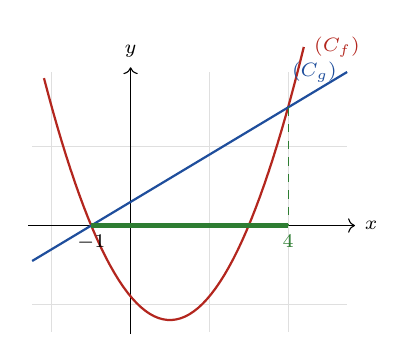
\begin{tikzpicture}[x=0.5cm,y=0.3cm,font=\scriptsize]
\draw[gray!25] (-2.5,-4.5) grid (5.5,6.5);
\draw[->] (-2.6,0)--(5.7,0) node[right]{$x$}; \draw[->] (0,-4.6)--(0,6.7) node[above]{$y$};
\draw[cThm,thick,domain=-2.2:4.4,samples=60] plot (\x,{\x*\x-2*\x-3}) node[right]{$(C_f)$};
\draw[cDef,thick] (-2.5,-1.5)--(5.5,6.5) node[left]{$(C_g)$};
\draw[cRem,dashed] (-1,0)--(-1,0) (4,5)--(4,0) node[below]{$4$};
\node[below] at (-1,0){$-1$};
\draw[cRem,line width=1.6pt] (-1,0)--(4,0);
\end{tikzpicture}\end{LTR}\par}{50 د}{نقارن الحل البياني بالجبري.}
\Row{}{%
\Lab{cThm!80!black}{حذار}\ الحل البياني تقريبي: نتحقق جبرياً.}{}{}
\Row{التقويم}{%
\Lab{cEx}{تطبيق}\par $f(x)=x^2$ و $g(x)=2x+3$. حل بيانياً ثم جبرياً $f(x)=g(x)$ و $f(x)>g(x)$.\par\textbf{الحل:} $x^2-2x-3=(x-3)(x+1)$: $\{-1;3\}$ ؛ $]-\infty;-1[\cup]3;+\infty[$.\par\textbf{واجب منزلي:} تمارين من الكتاب المدرسي.\par\smallskip\textbf{ملاحظات حول سير الحصة:} \dotfill}{25 د}{تقويم فردي.}
\end{Sayr}
\newpage
\ModhHead{35}{1 ج م ع ت}{جبر}{العبارات الجبرية}{02 سا}{ترييض المشكلات: معادلات ومتراجحات من الدرجة الأولى والثانية}%
{\begin{itemize}\item حل معادلات ومتراجحات.\end{itemize}}%
{\begin{itemize}\item ترييض وضعية بمعادلة أو متراجحة.\item حل مشكلات ومناقشة الحلول.\end{itemize}}%
{المنهاج ، الكتاب المدرسي ، مراجع ، الحاسبة البيانية.}
\begin{Sayr}
\Row{مرحلة الانطلاق}{%
\textbf{التهيئة النفسية:} «عدد مربعه يساوي ضعفه»: ما هو؟}{10 د}{لغز شفهي.}
\Row{التشخيص والاكتشاف}{%
\Lab{cEx}{وضعية مقترحة}\par مستطيل محيطه $34$ m ومساحته $60$ m². ما بعداه؟\par\ck\ نسمي $x$ أحد البعدين ، فالآخر $17-x$.\par
\ck\ $x(17-x)=60\iff x^2-17x+60=0$ ؛ $\Delta=49$ ، $x=12$ أو $x=5$.\par
\ck\ البعدان $12$ m و $5$ m.\par
}{35 د}{عمل في مجموعات.}
\Row{بناء المعارف}{%
\Lab{cMeth}{مراحل الترييض}\par\ck\ اختيار المجهول وتحديد مجموعة قيمه الممكنة.\par
\ck\ ترجمة المعطيات إلى معادلة أو متراجحة.\par
\ck\ الحل ، ثم مناقشة الحلول المقبولة حسب الوضعية.\par
\Lab{cEx}{مثال}\par\ck\ عددان طبيعيان متتابعان جداؤهما $156$: $n(n+1)=156$ ، $n=12$ (نرفض $-13$): العددان $12$ و $13$.\par
\ck\ حديقة مربعة يحيط بها ممر عرضه $1$ m ، المساحة الكلية $64$ m²: $(x+2)^2=64$ ، $x=6$ m.\par
}{50 د}{نكتب مراحل الترييض على السبورة.}
\Row{}{%
\Lab{cThm!80!black}{حذار}\ نتحقق أن الحل يناسب الوضعية (طول موجب ، عدد طبيعي $\ldots$).}{}{}
\Row{التقويم}{%
\Lab{cEx}{تطبيق}\par\Num{1} عيّن عددين مجموعهما $10$ وجداؤهما $21$. \Num{2} ما قيم $x$ التي تجعل مساحة مربع ضلعه $x$ أكبر من محيطه؟\par\textbf{الحل:} \Num{1} $t^2-10t+21=0$: $3$ و $7$ ؛ \Num{2} $x^2>4x$ و $x>0$: $x>4$.\par\textbf{واجب منزلي:} تمارين حوصلة المحور من الكتاب المدرسي.\par\smallskip\textbf{ملاحظات حول سير الحصة:} \dotfill}{25 د}{نهاية المحور: فرض أو تمارين حوصلة.}
\end{Sayr}
\end{document}
